% !TeX root = ../../../../thesis.tex


\subsection{Testbed}
\label{subsec:ac-testbed}

\begin{figure}[ht]
	\centering
	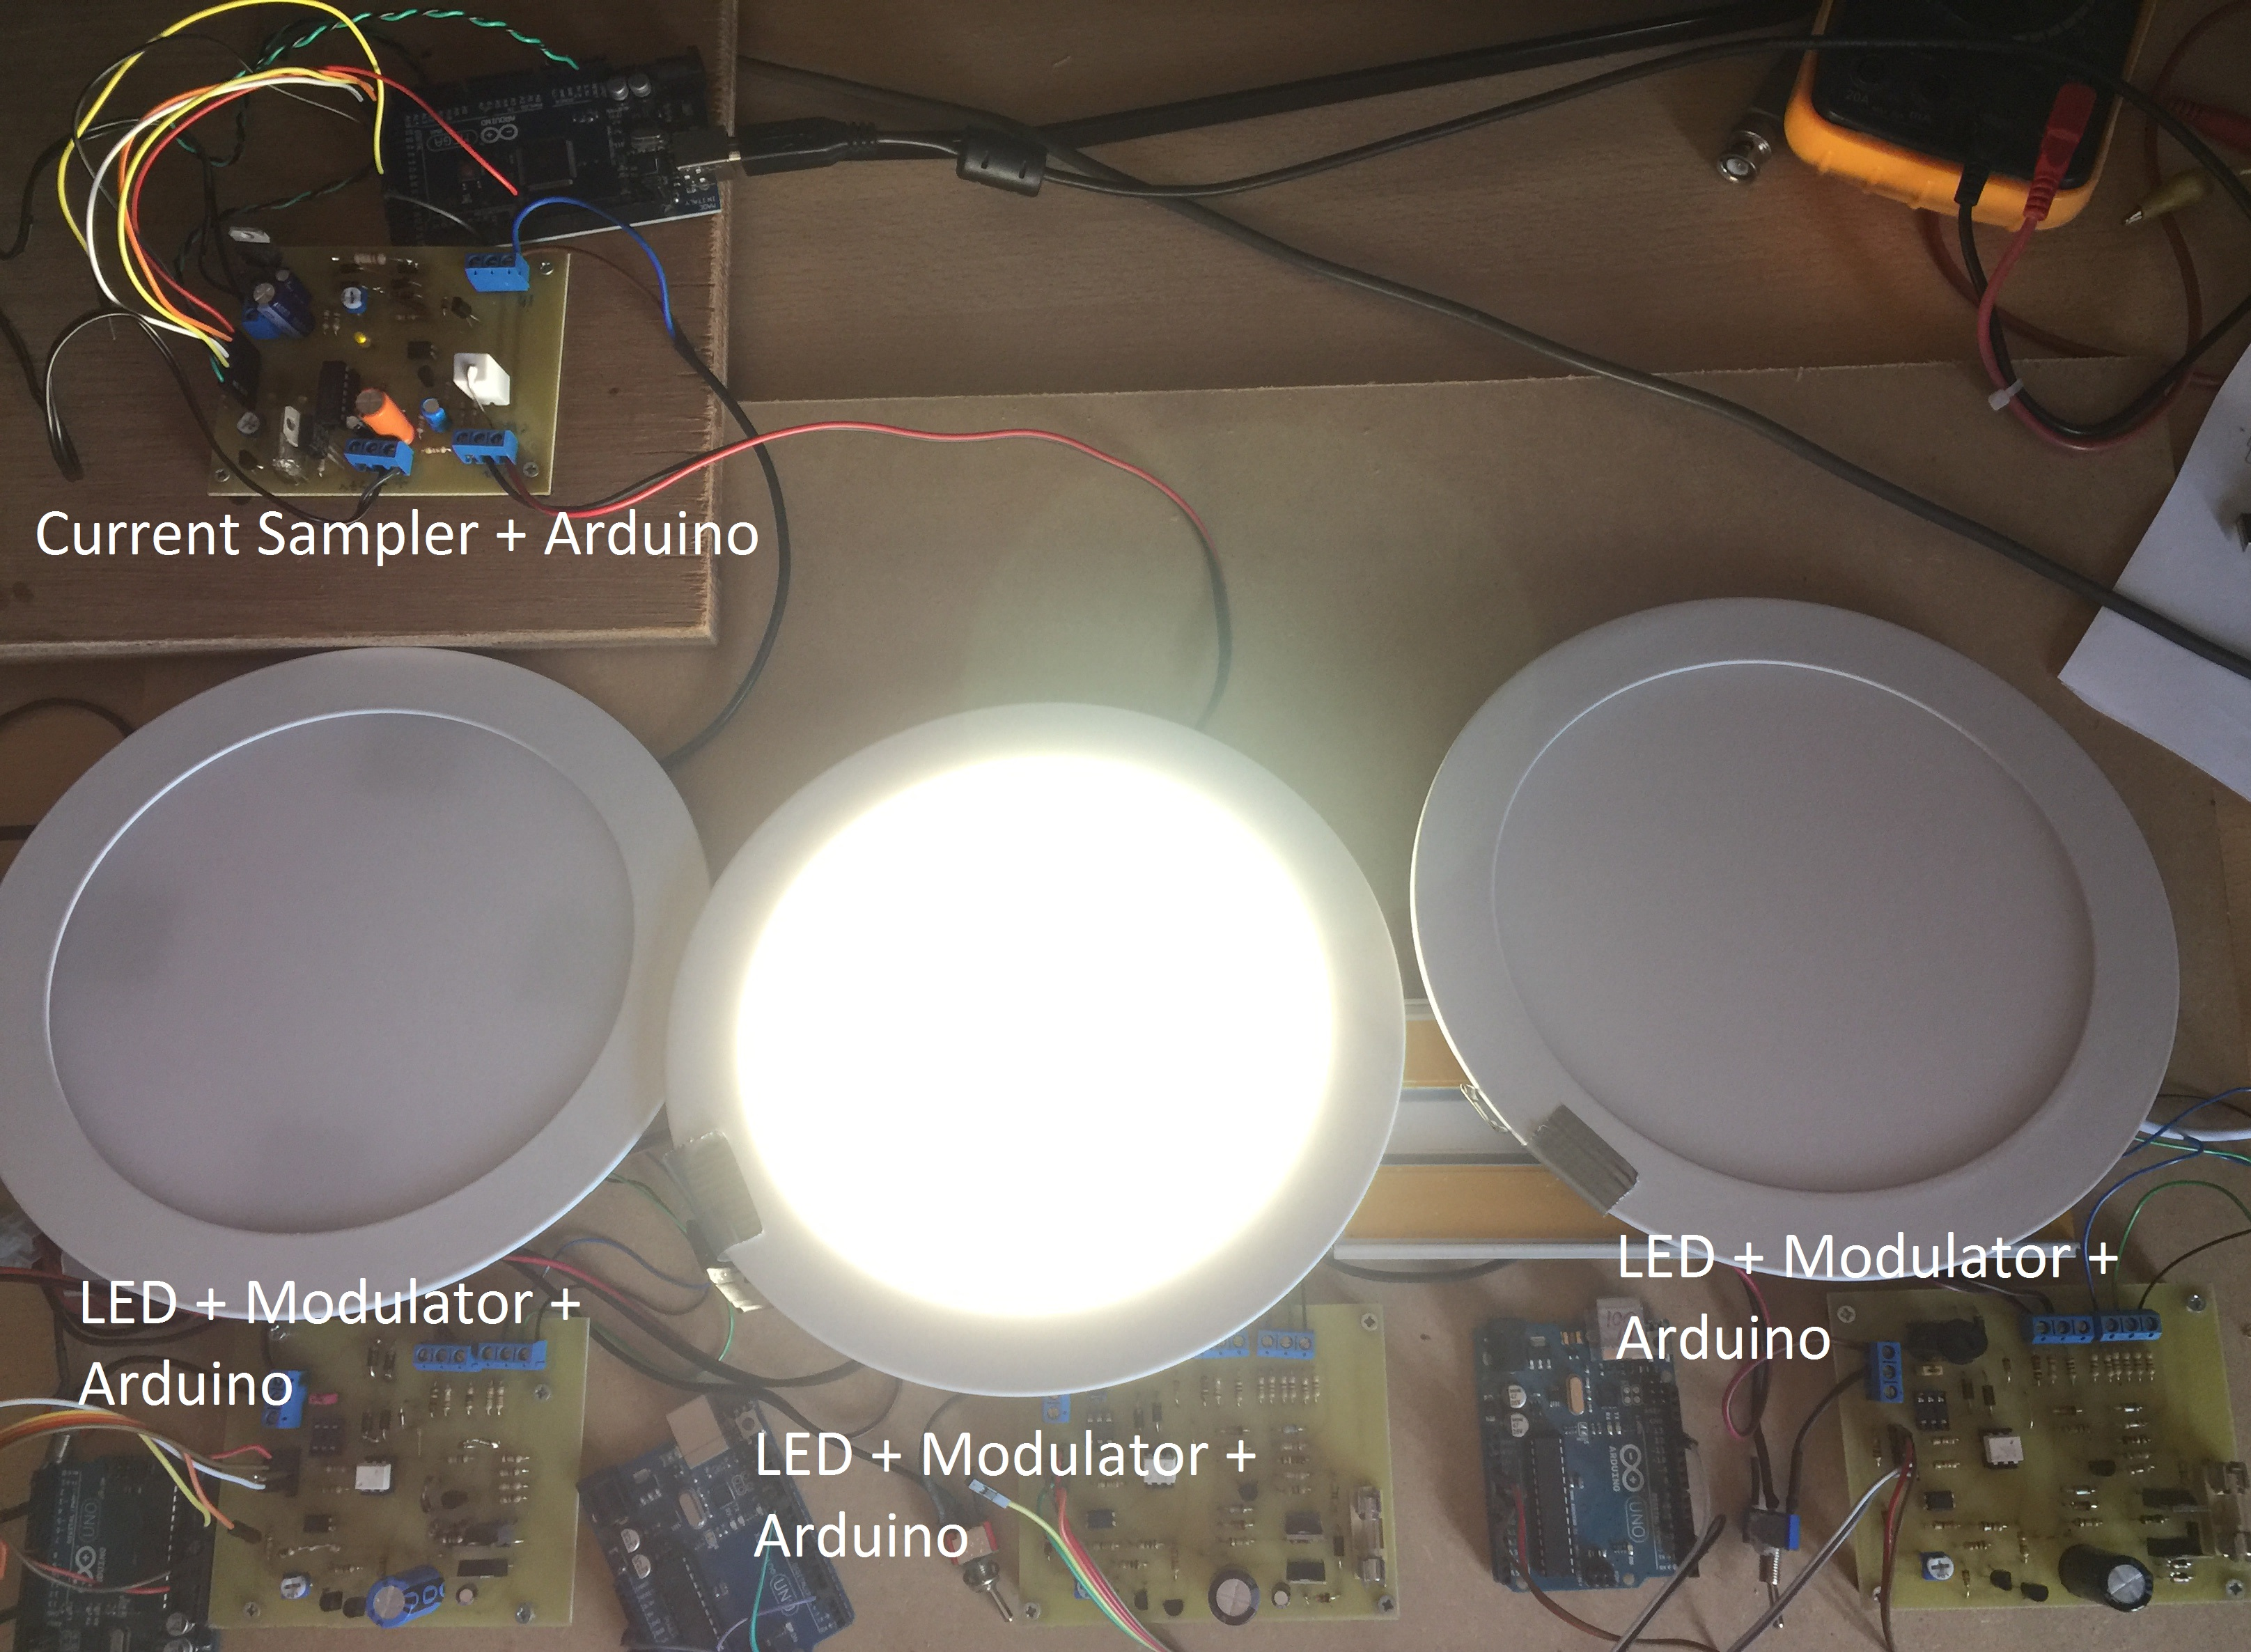
\includegraphics[angle=0,width=\textwidth,height=.9\textheight,keepaspectratio]{chapters/hardware-chapters/AC/ac-test-bed/ac-test-bed-picture}
	\caption{Picture of the AC testbed, consisting of three modulators each connected to three commercial LEDs. The modulators are controlled via three separate Arduino boards. Finally there is the current sampler with its own Arduino board.}
	\label{fig:ac-test-bed-picture}
\end{figure}



An overview of the AC testbed can be found in \autoref{fig:ac-test-bed-architectural-overview} and a picture of the actual testbed itself can be seen in \autoref{fig:ac-test-bed-picture}.
In the testbed three commercial LEDs are used which are powered by the custom modulators as explained in \autoref{subsec:ac-modulator}.
Arduino boards are controlling the modulators.
The modulators are connected in parallel. 
And the custom current-sampler is connected in series to measure the current and decode the information that the modulators encode into the current draw.
The custom current-sampler has its own Arduino board to process the current signal.
All Arduino board are stand-alone, and are not connected to each other in any way.


\begin{figure}[t]
	\centering
	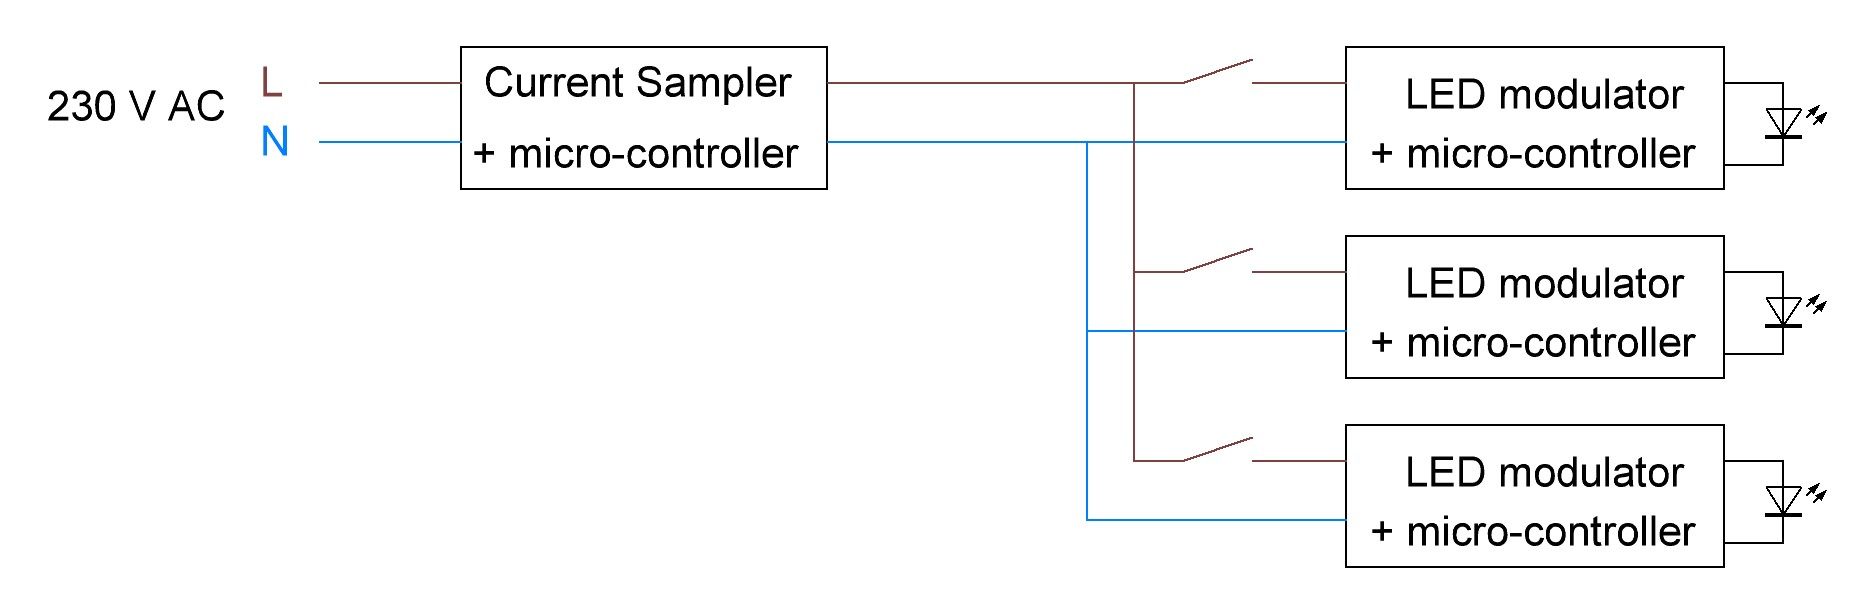
\includegraphics[angle=0,width=0.9\textwidth,keepaspectratio]{chapters/hardware-chapters/AC/ac-test-bed/ac-test-bed-architectural.JPG}
	\caption{Architectural overview of the AC testbed. Three LED modulators, with switches to turn the LED on and off, are connected in parallel with each other and in series with the current sampler.}
	\label{fig:ac-test-bed-architectural-overview}
\end{figure}



In \autoref{fig:raw-ac-testbed-adc-data-testbed} the raw data that is collected by the smart-meter can be seen.
The current signal is shown here alongside the trigger output.
In the raw data the charging peaks of the capacitor can be seen at timestamps: 5, 15 and 25 ms. %of the non-disturbing voltage source
Note that these peaks indeed do not interfere with the modulated data.
The modulated data and the charging peaks can be filtered out by the micro-controller with the help of the triggering circuits logical output.
As discussed in \autoref{subsec:ac-modulator}, the time that is available for modulation is 8 ms in a 10 ms period.
Depending on the length of the ID $L$ and the modulation frequency $f$, it can happen that this window of 8 ms is too small to encode the entire ID.
In this case, the remaining bits of the ID which could not fit inside the first 8 ms window, will be transmitted in the next window.
An evaluation with this testbed will be done in \autoref{subsec:ac-evaluation}.



\begin{figure}[ht]
  \centering
  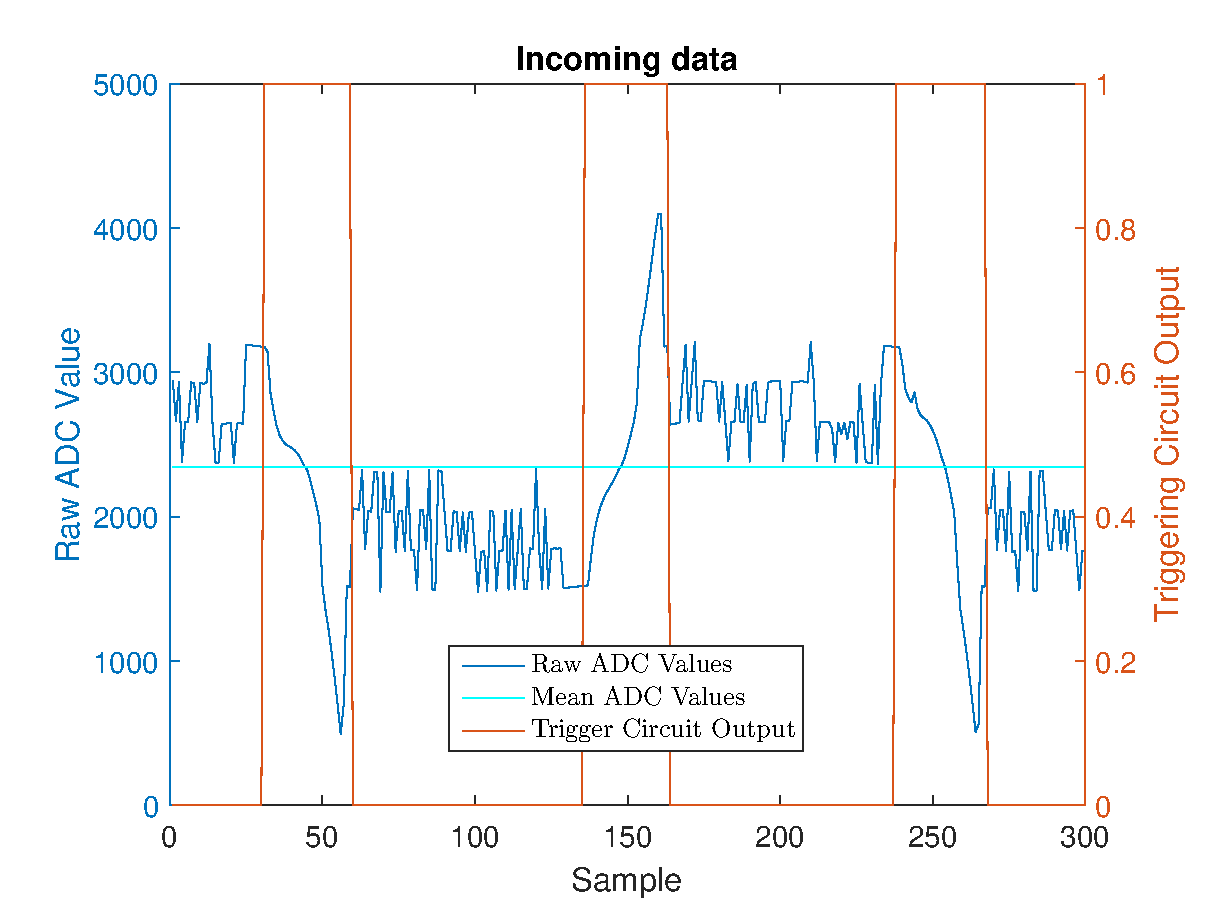
\includegraphics[width=0.7\textwidth]{chapters/evaluation-chapters/hardware/ac/raw-ac-testbed-adc-data.eps}
    \caption{Incoming data to the AC current sampler. The raw ADC values are plotted as well as the triggering circuit output.}
  \label{fig:raw-ac-testbed-adc-data-testbed}
\end{figure}

